\part{A Multi-Agent System for Optimization}

\chapter{Agent-Based Modeling and Simulation of an Optimization Problem}

[[Insister sur le découpage inhérent au problème (pas de réductionnisme)]]
[[utiliser un exemple en fil rouge -> Turbofan ?]]

\section{Problem Modeling with NDMO}\label{modeling}

[[A CHANGER: In answer to the previous shortcomings, we propose a generic approach called Natural Domain Modeling for Optimization (NDMO) that relies on a natural or intrinsic description of the problem (\textit{i.e.} close to the reality being described).]]

\begin{figure}[]
	\centering
	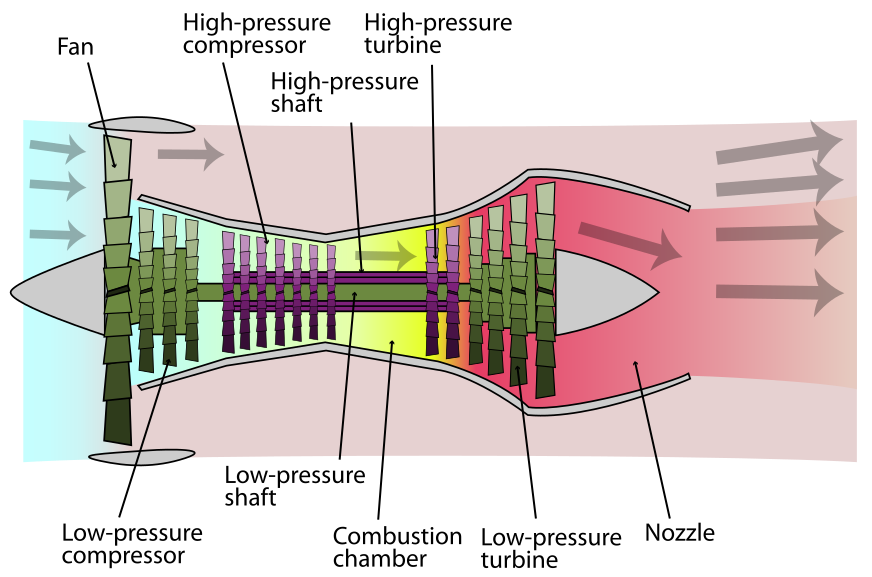
\includegraphics[width=0.8\textwidth]{Turbofan_operation}
	\caption{Illustration of a Turbofan engine (CC SA-BY  \href{http://en.wikipedia.org/wiki/File:Turbofan_operation.svg}{K. Aainsqatsi})}
	\label{turbofan_illu}
\end{figure}

To illustrate how an optimization problem is modeled, we use a simplified Turbofan optimization problem. On \figurename{} \ref{turbofan_illu}, an illustration of the principle of the turbofan can be seen. In this figure, the bypass ratio is the ratio between the air drawn in by the fan not entering engine core (which is \emph{bypassed}) and the air effectively used for the combustion process. The pressure ratio is the ratio between pressure produced by the compressors and the pressure it receives from the environment.

In order to identify the elements of a generic continuous optimization model, we worked with experts from several related fields: numerical optimization, mechanics as well as aeronautics and engine engineers. As a result, we identified five classes of interacting entities: \emph{models}, \emph{design variables}, \emph{output variables}, \emph{constraints} and \emph{objectives}. These entities and their relations are represented by the diagram in \figurename{} \ref{class_diag}, that we detail next.

\begin{figure}[t]
	\centering
	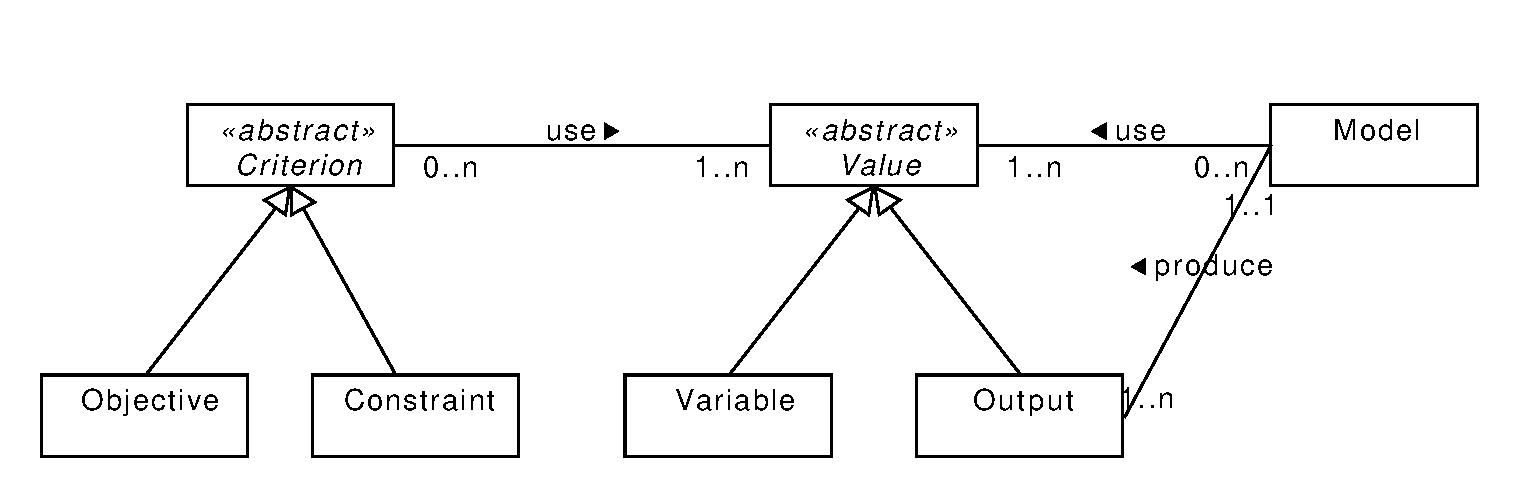
\includegraphics[width=0.9\textwidth]{class_diag}
	\caption{Class diagram of MDO problems}
	\label{class_diag}
\end{figure}

In \figurename{} \ref{turbofan:math}, the analytic expression of this optimization problem is given, while in \figurename{} \ref{turbofan:graph}, the problem is presented as a graph of the different entities. The design variables of this problem are $pi\_c$ and $bpr$, which indicate respectively the compressor pressure ratio and the bypass ratio of the engine. The turbofan model produces three outputs: $Tdm0$, $s$ and $fr$, representing respectively the thrust, fuel consumption and thrust ratio of the engine. In this problem we try to maximize the thrust and minimizing the fuel consumption while satisfying some feasibility constraints. 

\begin{figure}[]
\centering
\subfloat[mathematical formulation.]{\begin{minipage}{0.4\textwidth}
		$\begin{array}{c}
			(Tdm0, s, fr) = Turbofan(pi\_c, bpr) \\
			max \; Tdm0 \\
			min \; s \\
			subject \; to \\
			s \leq 155 \\
			fr \geq 4
		\end{array}$
\label{turbofan:math}
\end{minipage}}\hfill%
\subfloat[{corresponding entities graph.}]{\begin{minipage}{0.6\textwidth}%
		\centering
		\label{turbofan:graph}
		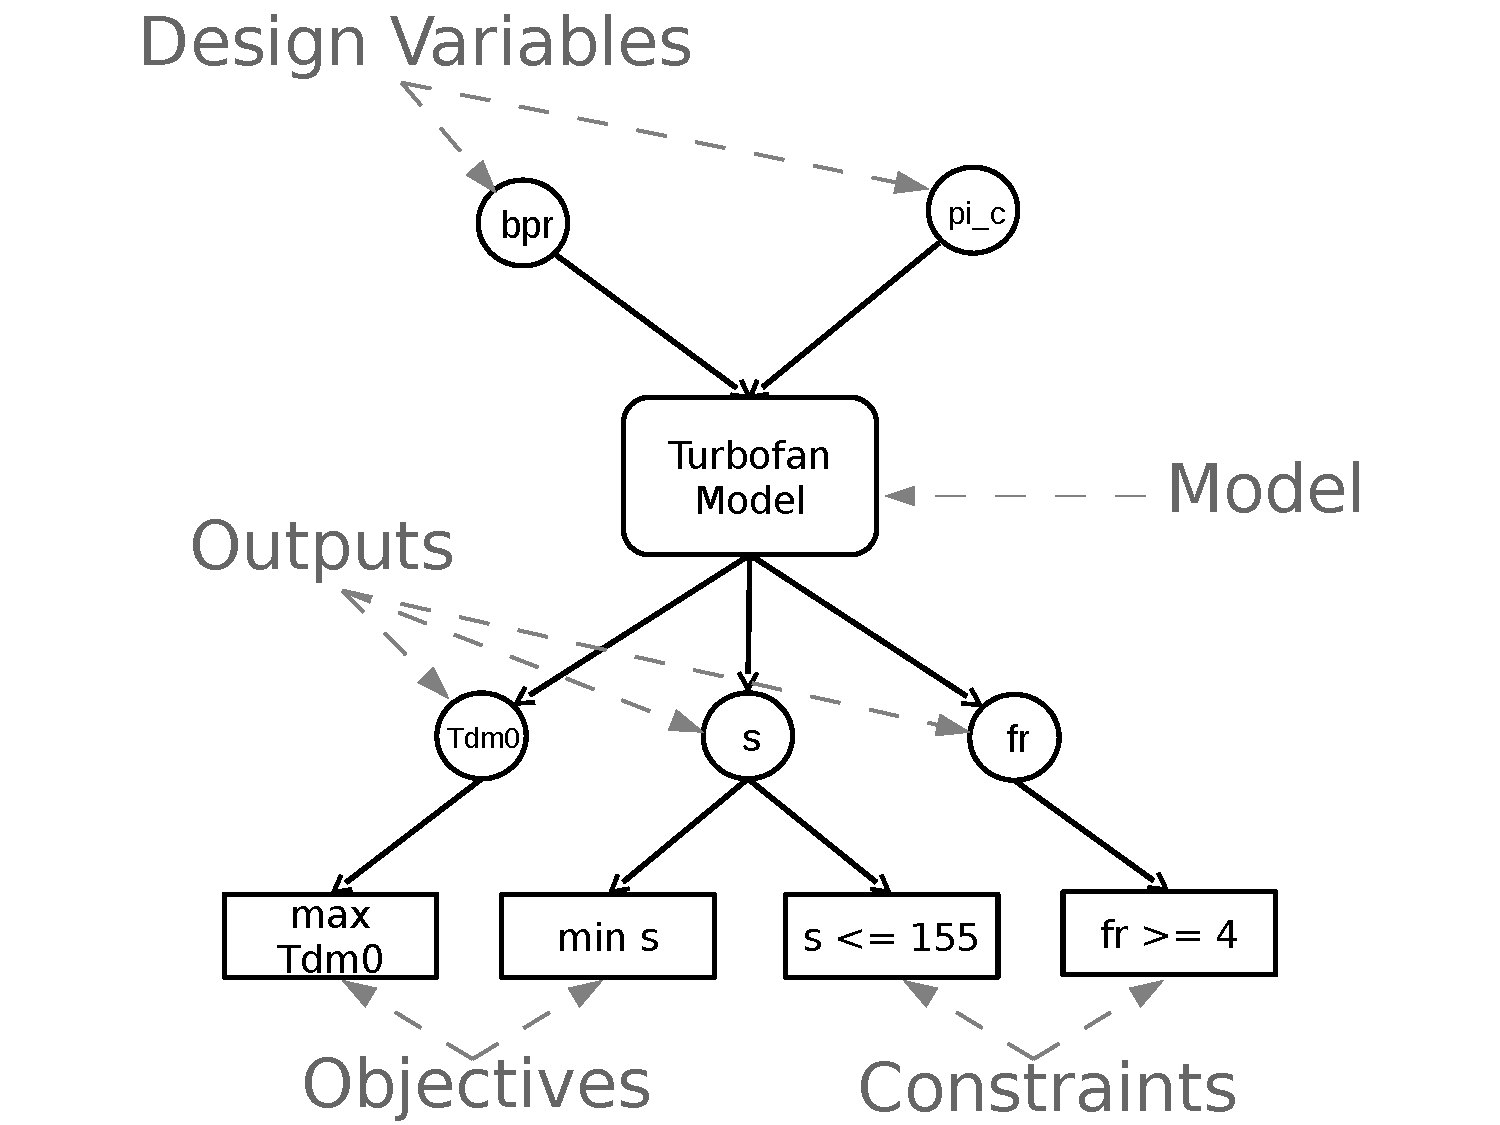
\includegraphics[width=\textwidth]{testcases-Turbofan-annoted}
\end{minipage}}

\caption{Turbofan problem.}
\label{turbofan}

\end{figure}

Let's now see in more details the roles of each of these fives entities: \emph{model}, \emph{variable}, \emph{output}, \emph{constraint} and \emph{objective}.

\subsubsection*{Models.}

In the most general case, a \emph{model} can be seen as a black box which takes input values (which can be \emph{design variables} or \emph{output variables}) and produces output values. A \emph{model} represents a technical knowledge of the relations between different parts of a problem and can be as simple as a linear function or a much more complex algorithm requiring several hours of calculation. Often some properties are known (or can be deduced) about a model and specialized optimization techniques can exploit this information.
In our Turbofan example, a \emph{model} entity is the $Turbofan$ function which calculate the three outputs using the values of $bpr$ and $pi\_c$.

\subsubsection*{Design Variables.}

These are the inputs of the problem and can be adjusted freely (within their defining boundaries). The goal is to find the set(s) of values for these variables that maximize the objectives while satisfying the constraints.
\emph{Design variables} are used by \emph{models} to calculate their outputs and by constraints and objectives to calculate their current value. A \emph{design variable} can be shared among several \emph{models}, objectives and constraints.
Keeping with our example, $bpr$ and $pi\_c$ are the two \emph{design variables} of our optimization problem.

\subsubsection*{Output Variables.}

These values are produced by a \emph{model}, and consequently cannot be changed freely.
As for the \emph{design variables}, the \emph{output variables} are used by \emph{models} to calculate their outputs and by constraints and objectives to calculate their current value.
In our example, $Tdm0$, $s$ and $fr$ are \emph{output variables} produced by the $Turbofan$ model.

\subsubsection*{Constraints.}

These are strict restrictions on some parts of the problem, represented as functional constraints defined by equalities and/or inequalities. These can be the expression of a physical constraint, or a requirement concerning the problem.
Regarding the Turbofan, the two \emph{constraints} are $s <= 155$ and $fr >=4$.

\subsubsection*{Objectives.}

The goals to be optimized. In the general case, different objectives are often contradictory.
The two \emph{objectives} of the Turbofan problems are to maximize $Tdm0$ and to minimize $s$.

Constraints and objectives are usually regrouped under the more general term of optimization criteria. 

\paragraph*{}
An interesting and important point is that both models, constraints and objectives involve computation. Often the most heavyweight calculus is encapsulated inside a model and the calculi concerning criteria tend to be simple equations, but this is neither an absolute requirement nor a discriminating characteristic.

The NDMO modeling aims to provide the most complete and natural representation of the problem. This modeling preserves the relations between the domain entities and is completely independent of the solving process. 

[[SAY IT IS A BIPARTITE GRAPH BETWEEN VALUES ENTITIES AND INTERNAL MODEL ENTITIES]]

\section{From an Optimization Problem to a Multi-Agent System}

Based on the NDMO modeling in section \ref{modeling}, we propose a multi-agent system where each domain entity is associated with an agent. Thus the multi-agent system is the representation of the problem to be solved with the links and communication between agents reflecting the natural structure of the problem. It is worth underlining the fact that this transformation (\textit{i.e.} the agentification) can be completely automatic as it is fully derived from the expression of the problem.

\begin{figure}
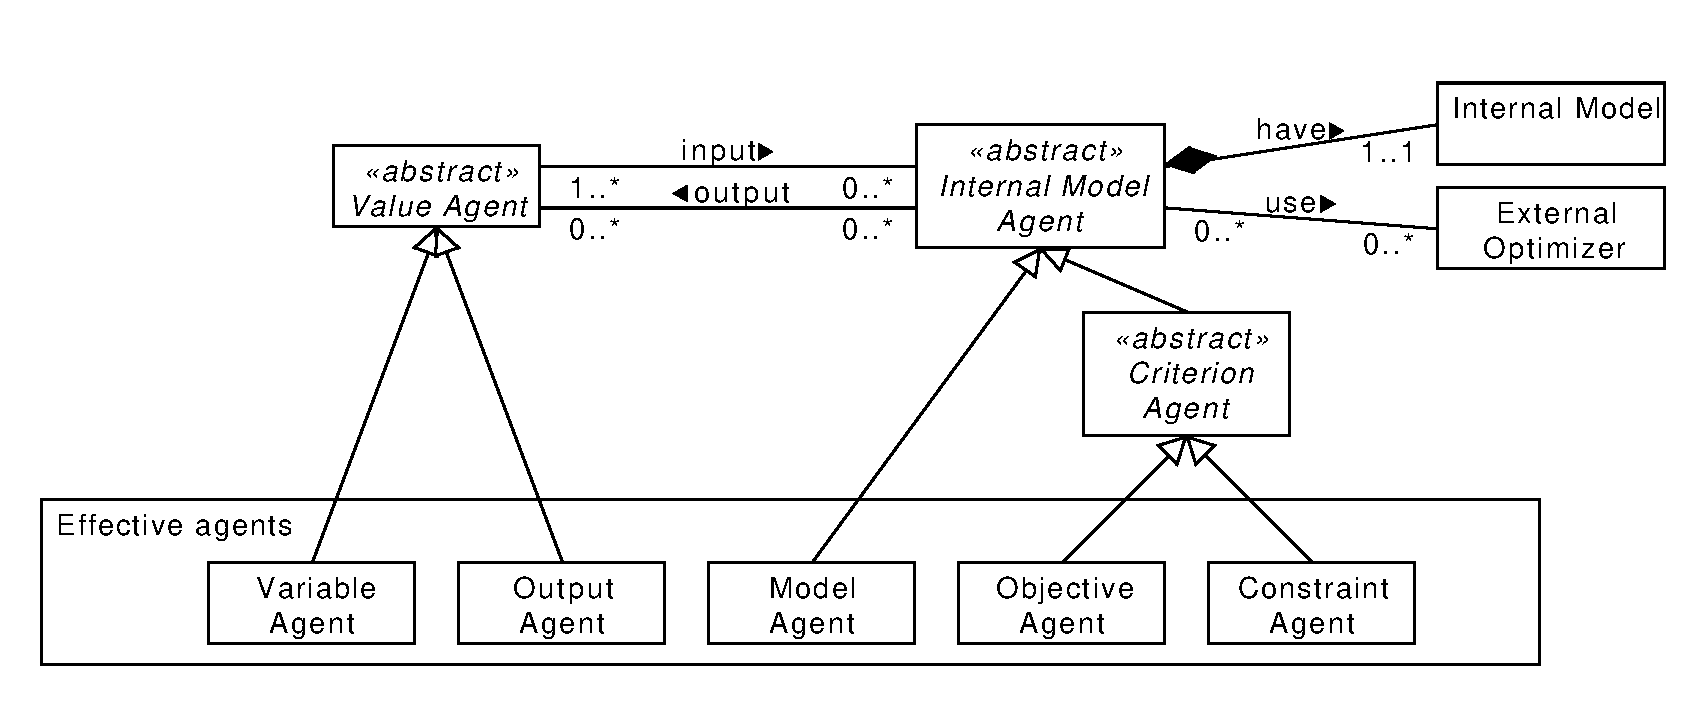
\includegraphics[width=\textwidth]{agent_class_diag}
\caption{System class diagram}\label{SMA_class_diagram}

\end{figure}

The solving process - constituted by the collective behavior of the agents - basically relies, on change-value requests sent by the criteria agents resulting in cooperatively decided adjustments done by the \emph{design variables} and on new values computed by the models resulting on the satisfaction or dissatisfaction of the criteria agents. 
In the same way we presented the different elements of NDMO, we now detail the behaviors of our five agent types: \emph{model}, \emph{variable}, \emph{output}, \emph{constraint} and \emph{objective} agents.
A summary of the basic principles of each agent type is given in Algorithm \ref{agent_algo}.

\subsubsection*{Model Agent.}

A \emph{model agent} takes charge of a model of the problem. It interacts with the agents handling its inputs (which can be \emph{variable} or \emph{output agents}) and the \emph{output agents} handling its outputs. Its individual goal is to maintain the consistency between its inputs and its outputs. To this end, when it receives a message from one of its inputs informing it of a value change, a \emph{model agent} recalculates the outputs values of its model and informs its\emph{output agents} of their new value. On the other part, when a \emph{model agent} receives a message from one of its \emph{output agents} it translates and transmits the request to its inputs. 

To find the input values corresponding to a specific desired output value, the \emph{model agent} uses an external optimizer. This optimizer is provided by the engineer based on expert domain-dependent knowledge regarding the structure of the model itself.
It is important to underline that the optimizer is used only to solve the local problem of the \emph{model agent}, and is  not used to solve the problem globally.


%\begin{algorithm}
%\caption{Behavior of a Model Agent}
%\begin{algorithmic}
%\While{running}
%	\State Receive Messages
%	\If{received new informs}
%        \State recalculate outputs
%        \State inform output agents
%    \EndIf      
%	\If{received new requests}
%       \State  use optimizer to find adequate inputs
%        \State propagate requests to input agents
%    \EndIf
%\EndWhile
%\end{algorithmic}
%\end{algorithm}

\subsubsection*{Variable Agent.}

This agent represents a \emph{design variable} of the problem. Its individual goal is to find a value which is the best equilibrium among all the requests it can receive (from models and criteria for which it is an input). The agents using the variable as input can send to it request asking to change its value. When changing value, the agent informs all agents linked to it of its new value. 

%\begin{algorithm}
%\caption{Behavior of a Variable Agent}
%\begin{algorithmic}
%\While{running}
%	\State Receive Messages  
%	\If{received new requests}
%       \State select most important
%       \State adjust value
%       \State inform related agents
%    \EndIf
%\EndWhile
%\end{algorithmic}
%\end{algorithm}

To find its new value, the \emph{variable agent} uses an exploration strategy based on \emph{Adaptive Value Trackers} (AVT)\cite{Lemouzy_2011}. The AVT can be seen as an adaptation of dichotomous search for dynamic values. The main idea is to change value according to the direction which is requested and the direction of the past requests. While the value varies in the same direction, the variation delta is increased so the value varies more and more. As soon as the requested variation changes, it means that the variable went past the good value, so the variation delta is reduced.

%While changing value based not on the value requested but on the direction can seem paradoxical, it must be recalled that, since no agent has a global view of the system, the requests made by the agents is often approximate, so the agents need to iterate many times. If the search space in large, the system could take time to converge towards the solution. By using a near-dichotomous strategy, we greatly accelerate this convergence.

This capability to take into account a changing solution allows the \emph{variable agent} to continuously search for an unknown dynamic target value. This capability is also a requirement for the system to be able to adapt to changes made by the engineer during the solving process.

\subsubsection*{Output Agent.}
The \emph{output agent} takes charge of an output of a model. \emph{Output agent} and \emph{variable agents} have similar roles, except \emph{output agents} cannot directly change their value. Instead they send a request to the \emph{model agent} they depend on. In this regard, the \emph{output agent} act as a filter for the \emph{model agent} it depends on, selecting among the different requests the ones it then transmits.

%\begin{algorithm}
%\caption{Behavior of an Output Agent}
%\begin{algorithmic}
%\While{running}
%	\State Receive Messages
%	\If{received new informs}
%        \State update its value
%        \State inform related agents
%    \EndIf      
%	\If{received new requests}
%       \State  select most important
%        \State transmit selected request to model agent
%    \EndIf
%\EndWhile
%\end{algorithmic}
%\end{algorithm}

As we will see in the next section, the \emph{output agent} is distinct from the \emph{variable agent} in the way that it can be involved in cycles. A cycle is a situation of interdependent models (that is, models which depend of each other to calculate their outputs).

%We describe in the next section the main difficulties when solving an optimization problem including interdependencies, and how can an \emph{output agent} detect and handle them.

\subsubsection*{Constraint Agent.}
 \emph{The constraint agent} has the responsibility for handling a constraint of the problem. When receiving a message from one of its inputs, the agent recalculates its constraint and checks its satisfaction. If the constraint is not satisfied, the agent sends \emph{change value} requests to its inputs.

%\begin{algorithm}
%\caption{Behavior of a Constraint/Objective Agent}
%\begin{algorithmic}
%\While{running}
%	\State Receive Messages
%	\If{received new informs}
%        \State update its value
%        \State use optimizer to find adequate inputs
%        \State send new requests to input agents
%    \EndIf      
%\EndWhile
%\end{algorithmic}
%\end{algorithm}

It should be noted that, to estimate the input values required to satisfy the constraint on its computed value, this agent employs the same technique as the \emph{model agent} (\textit{i.e.} an external optimizer).

\subsubsection*{Objective Agent.}
The  \emph{objective agent} is in charge of an objective of the problem. This agent sends requests to its inputs aiming to improve its objective, and recalculates the objective when receiving  \emph{value changed} messages from its inputs.

This agent uses an external optimizer to estimate input values which would improve the objective, as the model and constraint agents.


\chapter{Agents Behavior}

We will now discuss the behavior the the five agent types identified in the previous chapter. The functioning of the system can be divided into two main tasks: problem simulation and collective solving.

Problem simulation can be seen as the equivalent of the analysis of classical MDO method. The agents behavioral rules related to problem simulation concern the propagation of the values of design variables to the models and criteria based on the value. For this part, the agents will exchange \emph{inform} messages which contains calculated values. The "message flow" is top-down: the initial inform messages will be emitted by the variable agents and will be propagated down to the criteria agents. The illustration of the messages flow of simulation is shown on \figurename{} \ref{messages_flow:inf}.

Collective solving concerns the optimization of the problem. The agent behavioral rules related to collective solving are about satisfying the constraints while improving the objectives. For this part, the agents will exchange \emph{request} messages which contains desired variations of values. The "message flow" is bottom-up: the initial request messages will be emitted by the criteria agents and propagated up to variable agents. The illustration of the messages flow of solving is shown on \figurename{} \ref{messages_flow:req}.

\begin{figure}[h]
	\subfloat[Informs flow for simulation]{\begin{minipage}{0.4\textwidth}%
		\centering
		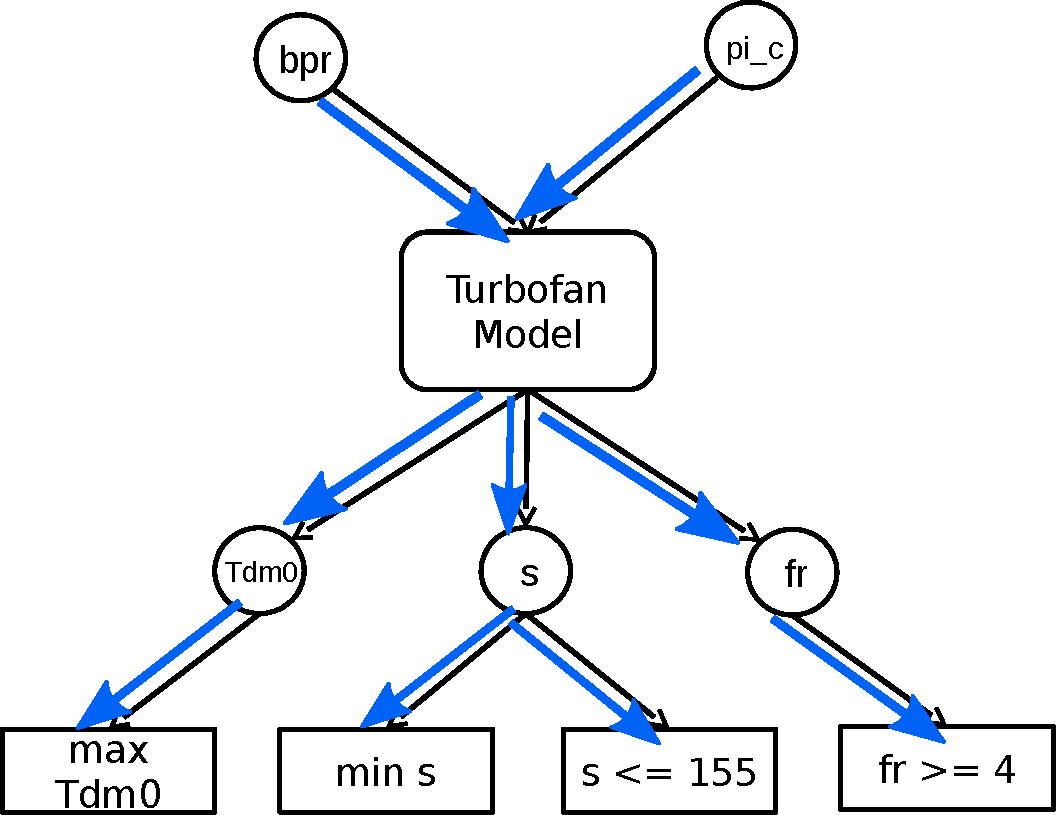
\includegraphics[width=\textwidth]{testcases-Turbofan-informs}
		\label{messages_flow:inf}
	\end{minipage}}
	\hfill
  	\subfloat[Requests flow for solving]{\begin{minipage}{0.4\textwidth}%
		\centering
		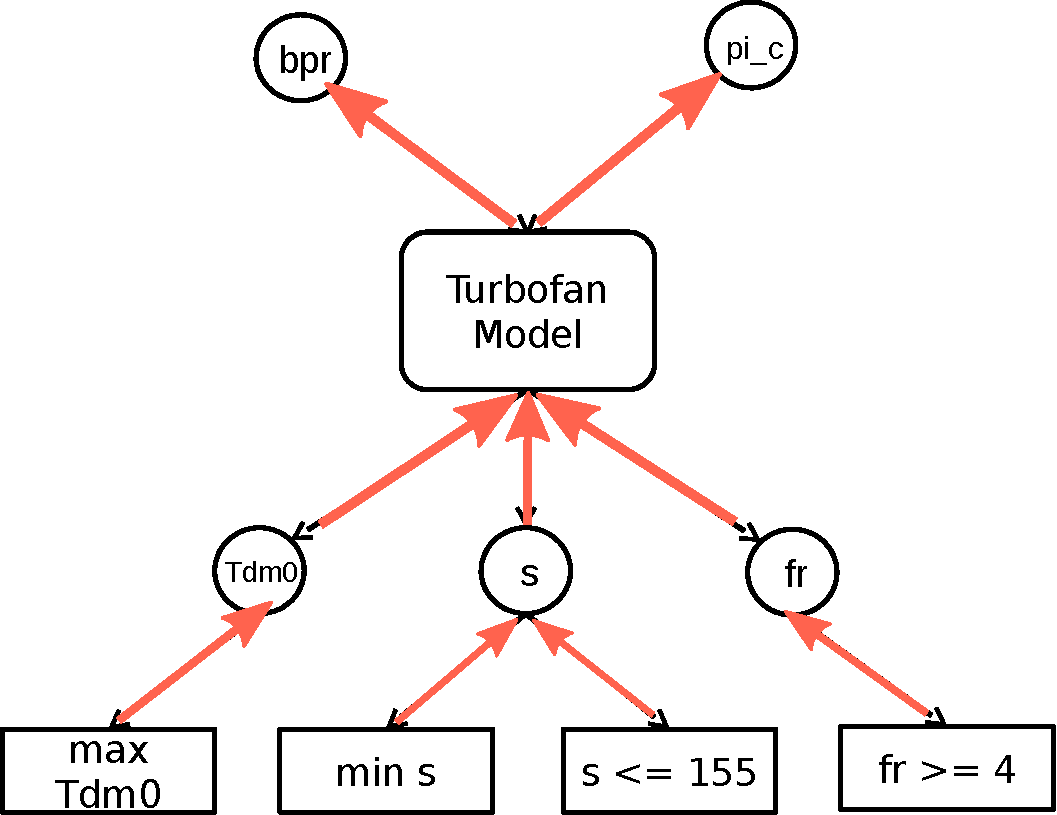
\includegraphics[width=\textwidth]{testcases-Turbofan-requests}
		\label{messages_flow:req}
	\end{minipage}}

	%new line
	\centering
	 \subfloat[Effective messages flow]{\begin{minipage}{0.4\textwidth}%
		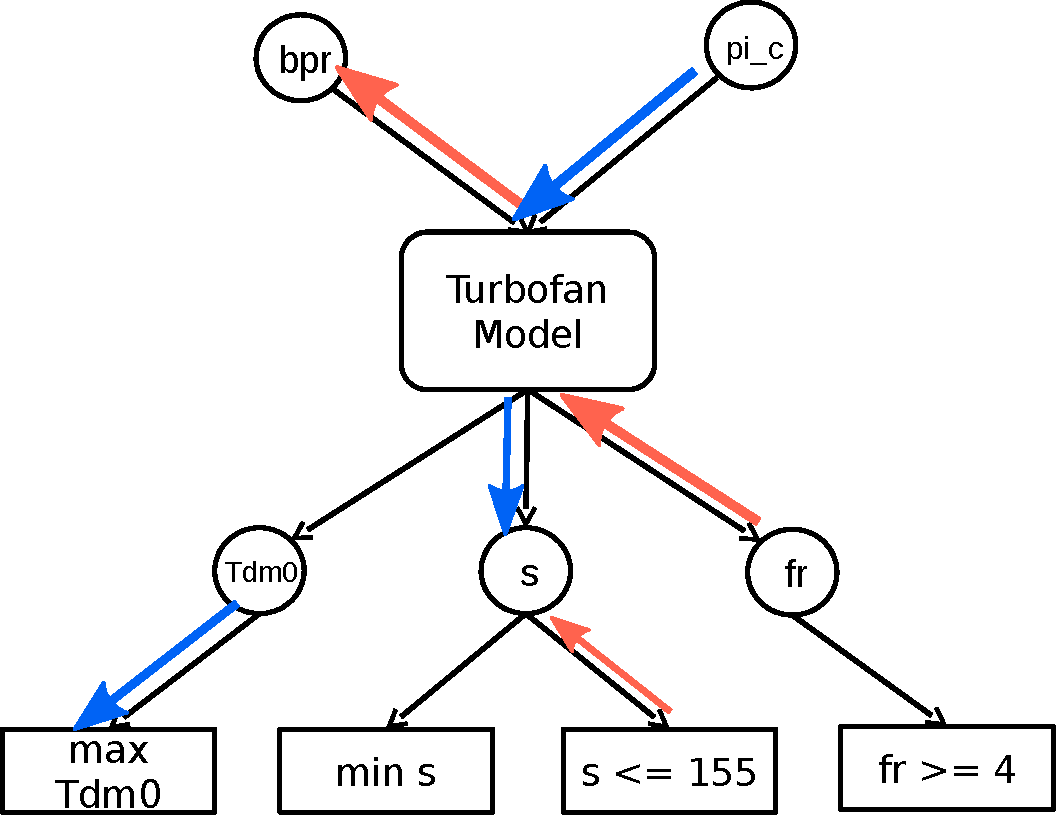
\includegraphics[width=\textwidth]{testcases-Turbofan-informs_requests}
		\label{messages_flow:eff}
	\end{minipage}}
	
	\caption{Messages flow for simulation and solving}
	\label{messages_flow}

\end{figure}

The agents behaviors regarding these two parts can be studied quite independently, we will thus present them separately.  It is however important to remember that these two parts are not executed separately. At runtime the agents will simulate the problem and solve it in parallel. Moreover, the different parts of the system will not necessarily work in a synchronous fashion. The effective messages flow of the system will more probably be akin to the \figurename{} \ref{messages_flow:eff}.

\section{Problem Simulation}

In this section we will present the agents behavior related to the simulation of the problem. Regarding this part, the main concern of the agents is to ensure consistency between the values of the design variables and the produced output. To this end, the agents will propagate \emph{Inform} messages through the system.

An inform message carry a new value $v$. The exact semantic of this information slightly changes depending on which agents are involved:

\begin{itemize}
\item If the message is sent from a value agent (variable or output) to a model or criterion agent, it indicates to the receiving agent that the sending agent has changed value.

\item If the message is sent from a model agent to an output agent, it indicates to the receiving agent that the model has calculated its new value.
\end{itemize}

In practice this distinction is not fundamentally important to understand the functioning of the system.

\subsection{Variable Agent}

Regarding problem simulation, the role of the variable agent is to ensure that the agents to which it is connected know its current value.
A variable agent has to send new Inform messages when:
\begin{compactitem}
\item new agents are connected to it (typically at the creation of the system)
\item it decided to change its value based on received requests (see \ref{collective_solv}[[CHANGE TO POINT DIRECTLY TO VARIABLE AGENT]])
\item the designer changed its value
\end{compactitem}

The behavior of the variable agent is resumed in algorithm \ref{algo_simulating_variable}.

\begin{algorithm}
\caption{Problem Simulation -Variable Agent Behavior}
\label{algo_simulating_variable}
\begin{algorithmic}
	$C \leftarrow$ previously connected output agents\;
	$C'\leftarrow$  newly connected output agents\;
		
	$v \leftarrow$ previous value\;
	$v'\leftarrow$ new value\;
	
	\tcp{notify contacts of value change}
	\If{$v \neq v'$}{
		$v \leftarrow v'$\;
		\ForEach{agent $a \in C$}{
			send($a$, new Inform($v$))\;
		}
	}
	
	\tcp{send its value to new contacts}
	\If{$C' \neq \emptyset$}{
		\ForEach{agent $a \in C'$}{
			send($a$, new Inform($v$))\;
		}
		$C \leftarrow C + C'$\tcp{memorize new outputs agents}
	}
	
\end{algorithmic}
\end{algorithm}

\subsection{Model Agent}

A model agent must maintain consistency between its inputs and outputs. When receiving an Inform message from one of the agents controlling its inputs, the model agent reevaluates its internal model taking the new value in account. Using the new values produced by the internal model, the model agents then send Informs messages to the agents responsible of its outputs.

All outputs of a model agent are not necessary associated with an ouput agent. For example, if the designer is not interested by the value represented by one of the outputs, he is not required to represent it by an agent. In this case the model agent will silently calculate the new value of the output at the same time than the others, but will not propagate it\footnote{Remember that the internal model of the agent is a black box, consequently the agent cannot choose to evaluate it partially. If the evaluation of the output could has been done independently from the others, it could be preferable to create two separate models}.

However, as the problem is dynamic, the designer can decide at any time to connect a new output agent to a previously unconnected output. In this case, the model agent must send to the output agent the last value it calculated for this output.

The behavior of the variable agent is resumed in algorithm \ref{algo_simulating_model}.

\begin{algorithm}
\caption{Problem Simulation -Variable Agent Behavior}
\label{algo_simulating_model}
\begin{algorithmic}
	$C \leftarrow$ previously connected output agents\;
	$C'\leftarrow$  newly connected output agents\;
	
	$\{v_i\} \leftarrow$ new input values\;
			
	\If{$\{v_i\} \neq \emptyset$}{
		$\{v_o\} \leftarrow$ previous output values\;
		$\{v'_o\}\leftarrow Model(\{v_i\})$\tcp{use internal model to recalculate outputs}
		\ForEach{agent $o \in C$}{
			\tcp{inform output agents of their new value}
			send($o$, new Inform($v'_o$))\;
		}
	}
	
	\tcp{Send their value to new outputs}
	\If{$C' \neq \emptyset$}{
		\ForEach{agent $o \in C'$}{
			send($o$, new Inform($v'_o$))\;
		}
		$C \leftarrow C + C'$\tcp{memorize new outputs agents}
	}
	
\end{algorithmic}
\end{algorithm}

\subsection{Output Agent}

\subsection{Constraint/Objective Agent}

\section{Collective Solving}\label{collective_solv}

During solving, the criteria agents try to improve their local goal. That is, the constraints agents try to keep their constraint satisfied, while the objective agents try to improve their objective. To this end they send \emph{Request} messages to the agents controlling their inputs, asking them to change value. The others agents have to propagate these requests toward the variable agents in the most adequate way.

\section{Non-Cooperative Situations}

\subsection{Conflicting Requests}

\subsection{Cooperative Trajectories}

\subsubsection{For Model Agents}

Models agents try to 

Let $M(I,O)$ be a model agent with a set of inputs $I$ and a set of output $O$.

Let $\{r = <\Delta_{o_{\in O}}^{r}, crit>\}$ be a set of  requests received for outputs $\{o\} \in O$, where $\Delta_{o}^{r}$ is the variation of output $o$ requested by $r$ and $crit$ the criticality of the request. By hypothesis, at most one request can concerns the same output.
Using an external optimizer, the agent obtains for each $r_k$ a set of corresponding input variations $\{\Delta_i^{r_k}\}_{i \in I}$.

For each input $i$ of the model, we need to select a variation.
First of all, we only keep the requested variations with the maximum criticality:  $\{\Delta_i^{r_{max}}\} \leftarrow \{\Delta_i^r : crit_r = max \{crit_{r \in R}\}\}$.
If $|\{\Delta_i^{r_{max}}\}| =  1$, then the agent knows which variation to request to the input agent.

Otherwise, the model agent will discriminate using the relative influence [[it learned | given by the analyser]] of the input on the outputs concerned by the requests: 
$\Delta_i^* \leftarrow \left\{ \Delta_i^{r_{max}} : r_{max} = argmax \frac{inf_{i,o_{r_{max}}}}{\sum \limits_{i \in I} inf_{i,o}} \right\}$

If at this step $|\Delta_i^*| >1$ [[then what?]]. Otherwise the unique $\Delta_i^*$ is selected.

\begin{algorithm}
\caption{Cooperative trajectory - Model agent}
\label{algo_cooperative_trajectory_model}
\begin{algorithmic}
	\ForEach{$i \in I_M$}{
		 $\{\Delta_i^{r_{max}}\} \leftarrow \{\Delta_i^r : crit_r = max \{crit_{r \in R}\}\}$\;
		 \eIf{$|\{\Delta_i^{r_{max}}\}| = 1$}{
		 	$\Delta_i^{r_{max}}$ is the variation requested to the input\;
		 }
		 {
			$\{\Delta_i^*\} \leftarrow \left\{ \Delta_i^{r_{max}} : r_{max} = argmax \frac{inf_{i,o_{r_{max}}}}{\sum \limits_ {i \in I} inf_{i,o}} \right\}$\;
		 }
	}
\end{algorithmic}
\end{algorithm}

\subsubsection{For Variable Agents}

\subsection{Cycle Solving}

\subsection{Hidden Dependencies}

\subsection{Asynchronous Requests}

\section*{}
The most important point is that each agent only has a local strategy. No agent is in charge of the optimization of the system as a whole, or even of a subset of the other agents. Contrary to the classical MDO methods presented earlier, the solving of the problem is not directed by a predefined methodology, but by the structure of the problem itself. The emerging global strategy is unique and adapted to the problem.

\begin{algorithm}
\caption{Agents Behaviors}\label{agent_algo}
\begin{algorithmic}

\SetKwProg{Bv}{behavior of }{}{}

\Bv{Model Agent}{
	\Repeat{resolution end}{
		analyze received messages\;
		\If{received new information messages}{
	        recalculate outputs\;
	        inform depending agents\;
	    }     
		\If{received new requests}{
	        use optimizer to find adequate inputs\;
	        propagate requests to input agents\;
	   }
	}
}

\Bv{Variable Agent}{
	\Repeat{resolution end}{
		analyze received messages\;
		\If{received new requests}{
	       select most important\;
	       adjust value\;
	       inform depending agents\;
	    }
	}
}

\Bv{Output Agent}{
	\Repeat{resolution end}{
		analyze received messages\;
		\If{received new information messages}{
	        update its value\;
	        inform depending agents\;
	    }      
		\If{received new requests}{
	        select most important\;
	        transmit selected request to model agent\;
	    }
    }
}

\Bv{Constraint/Objective Agent}{
	\Repeat{resolution end}{
		analyze received messages\;
		\If{received new information messages}{
	        update its value\;
	        use optimizer to find adequate inputs\;
	        send new requests to variable/output agents\;
	    }
	}
}
\end{algorithmic}
\end{algorithm}